\subsubsection{Differential Gears} \label{sec:Differentialgears}
The differential gear ensures that a minimal amount of the energy, received from the motor, is lost when the vehicle is turning. If one of the driving wheels brakes, the differential gears transfer the rotational energy from the braking side to the other side. This will minimize the loss of energy. The extra velocity, transferred to the opposite belt, makes the vehicle turn.

A differential gear system can be seen on \figref{diffGearLight}.

\begin{figure}[H]
	\centering
	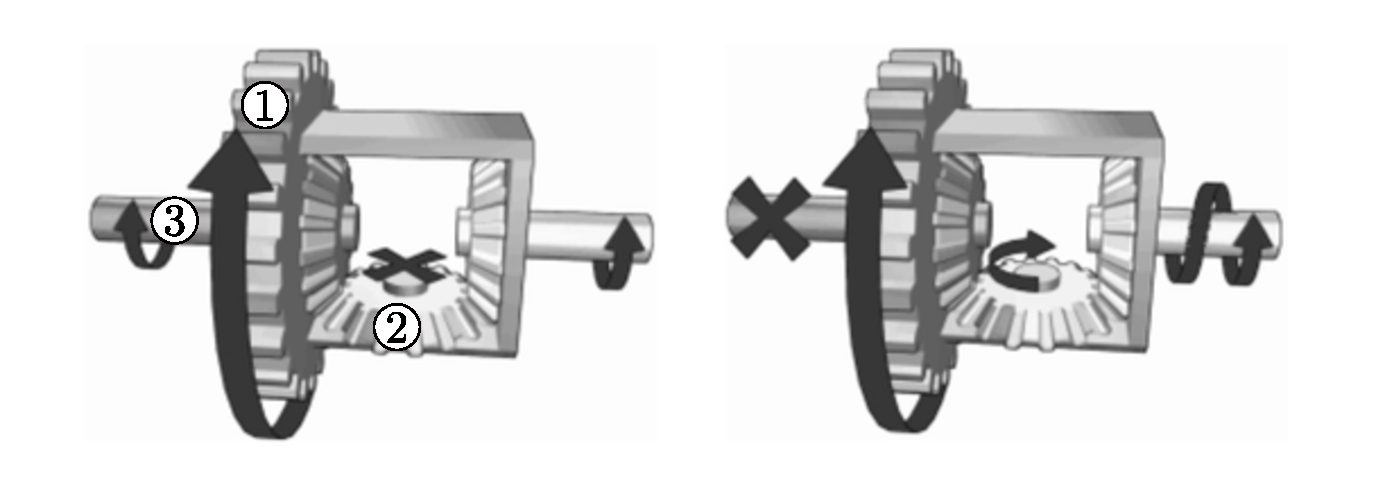
\includegraphics[scale=0.7]{figures/diffGearLightGray.pdf}
	\caption{Illustration of a differential gear system. On the left, the resistance on each side is equal, so the spider gear(2) does not rotate. On the right, the resistance on the left side is bigger than the one on the right side, so the spider gear rotates and transfers more rotational energy to the right side. \cite{MechanicalEngineering}}
	\label{diffGearLight}
\end{figure}

The differential gear system contains a ring gear (1), a spider gear (2), two side gears connected to the rest of the system (3) and a pinion gear (not shown on picture) connected to the ring gear. The pinion gear transfers the energy from the motor to the differential gear.

When the motor is running, the pinion gear transfers a rotational energy to the ring gear. The spider gear, fixed on to the ring gear, begins to rotate around the side gear. The ring gear is statically connected to the frame in which the spider gear is mounted. Therefore the transfer of rotation of the frame happens through the spider gear, which pushes on the side gears. If the resistance on both side gears is the same, see the left side in \figref{diffGearLight}, the same velocity is transferred to either side gear. Therefore the spider gear will not rotate around its own axis and apply the same rotational energy to each side gear.

When there is a difference in resistance on one side compared to the other, see the right side in \figref{diffGearLight}, one of the sides brakes and the spider gear will rotate. There is a bigger resistance on one side than on the other, so the side which is not braking will be easier to rotate. The ring gear and the spider gear are rotating at the same velocity around the two side gears. But the spider gear will apply less rotational velocity on the braking side than on the other side. In the case that the resistance on one side is infinite, the side gear on the none braking side will rotate twice as fast, compared to equal transfer of energy to the two sides.

Instead of only having one spider gear, as seen in \figref{diffGearLight}, there are two on the received vehicle, the functionality is the same, but two spider gears gives more reliability and solidity. 

%For the differential gear system on the vehicle, there is a more complete setup, shown on \figref{diffGearFull}
	%\caption{Illustration of the differential gear system on the vehicle \cite{MechanicalEngineering}}
%\begin{minipage}{\linewidth}
%      \centering
%      \begin{minipage}{0.65\linewidth}
%          \begin{figure}[H]
%              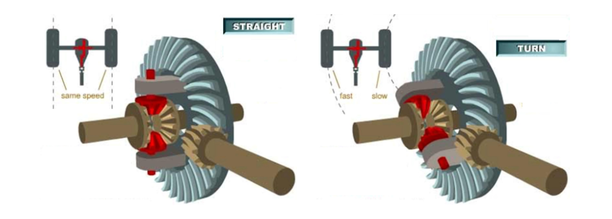
\includegraphics[width=0.95\textwidth]{figures/diffGearFull}
%              \caption{Illustration of the differential gear system placed on the received vehicle \cite{MechanicalEngineering}}
%              \label{diffGearFull}
%          \end{figure}
%      \end{minipage}
%      \hspace{0.05\linewidth}
%      \begin{minipage}{0.25\linewidth}
%      		\begin{enumerate}
%      			\item Pinion gear
%      			\item Ring gear
%      			\item Spider gears
%      			\item Side gears
%      		\end{enumerate}
%      \end{minipage}
%  \end{minipage}




%\begin{table} [H]
%\begin{tabular}{p{3cm} p{3cm}}

%\begin{figure}
%	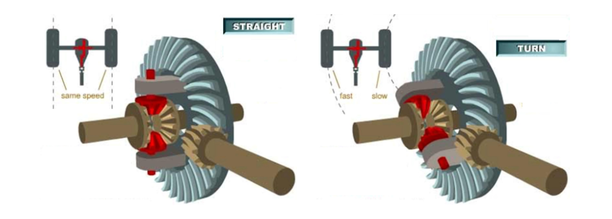
\includegraphics[scale=0.7]{figures/diffGearFull}
%	\label{diffGearFull}
%\end{figure}

%&

%\begin{enumerate}
 % \item Hallo
%\end{enumerate}

%\end{tabular}
%\end{table}

%\begin{figure} [h]
%	\centering
%	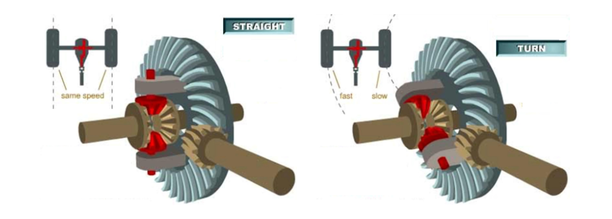
\includegraphics[scale=0.7]{figures/diffGearFull}
%	\caption{Illustration of the differential gear system on the vehicle \cite{MechanicalEngineering}}
%	\label{diffGearFull}
%\end{figure}

%The functionality of the differential gear is the same as with one spider gear. A gear shaft with is connected to the gear which gets rotated by the motor, is transferring the rotation from the motor to the ring gear(1). The spider gears(2) fixed on the ring gear rotates the side gears(3), in respect to the resistance affecting the side gears.

%\subsection{Things that maybe should be placed in this section}

%When a permanent magnet DC motor is used, the inductor and resistor in the motor causes a time constant, that the PWM time period should be less than:

%\begin{flalign}
%T &< 2 \cdot \frac{L_a}{R_a} \cdot ln(1-\frac{P}{100})\unit{s}
%\end{flalign}

%Where P is the duty cycle in percent, and La is the inductance in the motor, and Ra is the resistance in the motor.
